\hypertarget{attribute-driven-design}{%
\section{Attribute Driven Design}\label{attribute-driven-design}}


\begin{tcolorbox}[colback=blue!5!white,colframe=blue!75!black]
You’ll learn...
\begin{itemize}
    \item that quality attributes are main architectural drivers
    \item that tactics pave the way for the selection of architecture patterns
    \item and that Attribute Driven Design helps in finding the final architecture
\end{itemize}
\end{tcolorbox}

Idea:

\begin{itemize}
\tightlist
\item
  Beside functional and business requirements you consider also
  \textbf{quality requirements}
\item
  From the quality requirements \textbf{(quality attributes)} you choose
  among different sets of tactics
\item
  The selection of tactics helps you finding the architecture
\end{itemize}


Procedure
\begin{enumerate}
    \item Chose a Modul to decompose
    \item Refine this model
    \begin{enumerate}
        \item Choose Architectural drivers
        \subitem Quality, a Stimulus etc.
        \item Chose Style or Pattern that satisfies drivers $\rightarrow$ Child Modules
        \subitem for each quality there are tactics, for many tactics there are architectural styles/patterns
        \item allocate functionality to child modules from use cases
        \item define interfaces for child modules
        \item verify use cases and quality scenarios to be contraints for child modules
    \end{enumerate}
    \item Repeat Steps
\end{enumerate}





\hypertarget{quality-attributes}{%
\subsection{Quality attributes}\label{quality-attributes}}

\begin{itemize}
\tightlist
\item
  The notion of quality is central in software architecting: a software
  architecture is devised to gain insight in the qualities of a system
  at the earliest possible stage.
\item
  Some qualities are \textbf{observable} via execution: performance,
  security, availability, functionality, usability
\item
  And some are \textbf{not observable} via execution: modifiability,
  portability, reusability, {[}\ldots{}{]}, testability
\end{itemize}


\hypertarget{quality-attribute-scenario}{%
\subsubsection{Quality Attribute
Scenario}\label{quality-attribute-scenario}}

Quality attribute scenarios are a means to characterize quality
attributes. A quality attribute scenario is a quality-attribute-specific
requirement. It consists of six parts:

\begin{enumerate}
\def\labelenumi{\arabic{enumi}.}
\tightlist
\item
  Source of stimulus (Anregung, Anstoss)\\
  a human, another computer, another actuator
\item
  Stimulus\\
  a sort of an event such as: a crash, an unexpected message, change
  request, \ldots{}
\item
  Environment\\
  operating condition of the system such as ``normal mode'',
  ``overloaded''
\item
  Artifact\\
  the ``thing'' that is stimulated (the system, a process, a component,
  \ldots{})
\item
  Response\\
  an activity undertaken after arrival of the stimulus
\item
  Response measure something measurable upon completion of the response
  activity (down time, \ldots{})
\end{enumerate}

General quality attribute scenarios are

\begin{itemize}
\tightlist
\item
  system independent
\item
  can potentially be relevant for any system
\end{itemize}

\begin{figure}[H]
\centering
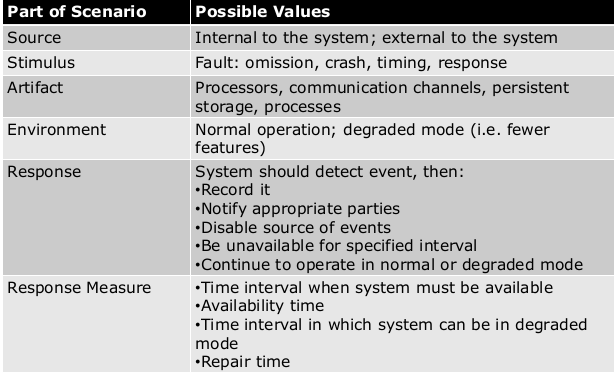
\includegraphics[width=0.5\textwidth]{figures/qualityScenarioGeneral.png}
\caption{General Quality Scenario}
\end{figure}


Concrete quality attribute scenarios are

\begin{itemize}
\tightlist
\item
  specific to a particular system under consideration
\end{itemize}

\begin{figure}[H]
\centering
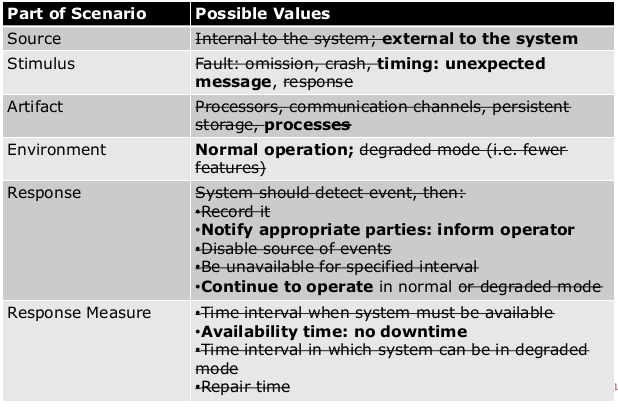
\includegraphics[width=0.5\textwidth]{figures/qualityScenarioConcrete.png}
\caption{Concrete Quality Scenario}
\end{figure}

\hypertarget{concrete-attribute-generation}{%
\subsubsection{Concrete Attribute
Generation}\label{concrete-attribute-generation}}

From the requirements elicitation above:

\begin{itemize}
\tightlist
\item
  choose one or more entries
\item
  from each column of the XX general scenario table, where XX stands for

  \begin{itemize}
  \tightlist
  \item
    availability
  \item
    modifiability
  \item
    performance
  \item
    securitytesting
  \item
    usability
  \end{itemize}
\item
  Add minor modifications to make your choice more readable
  -\textgreater{} concrete particular scenario
\item
  Repeat this step for each relevant quality attribute.
\end{itemize}

\subsubsection{Sample Modifiability Scenario}
\begin{figure}[H]
\centering
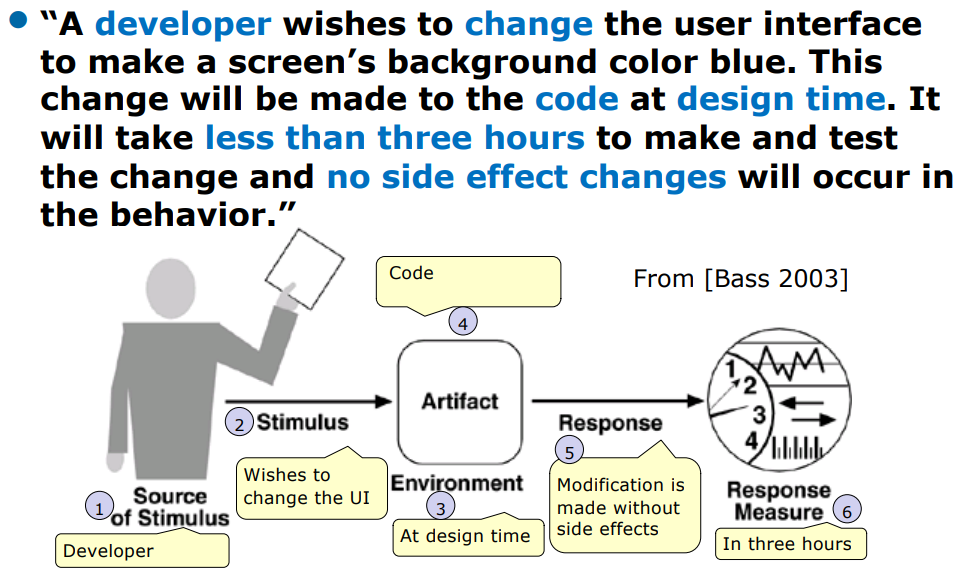
\includegraphics[width=0.5\textwidth]{figures/Wish.PNG}
\caption{Sample Modifiability Scenario}
\end{figure}


\clearpage
\hypertarget{tactics}{%
\subsection{Tactics}\label{tactics}}

Given the derived quality attribute scenarios, determine the
(architectural) tactics\ldots{}

Kinds of tactics:

\begin{itemize}
\tightlist
\item
  availability tactics
\item
  modifiability tactics
\item
  performance tactics
\item
  security tactics
\item
  testability tactics
\item
  usability tactics
\end{itemize}

Tactics determine architectural patterns or styles

\hypertarget{what-is-a-tactic}{%
\subsubsection{What is a tactic}\label{what-is-a-tactic}}

A tactic is a design decision that influences the control of a quality
attribute response.

\begin{figure}[H]
\centering
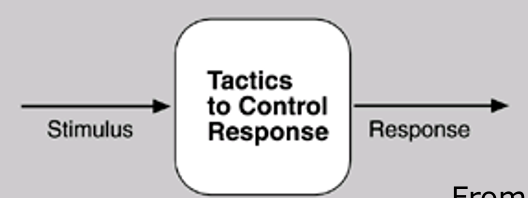
\includegraphics[width=0.4\textwidth]{figures/tactic.png}
\caption{Tactic}
\end{figure}

\hypertarget{example-on-modifiability-tactic}{%
\subsubsection{Example on Modifiability
Tactic}\label{example-on-modifiability-tactic}}

e.g.~The Goal of Modifiability tactics is to control time and cost to
implement, test, and deploy changes

\begin{figure}[H]
\centering
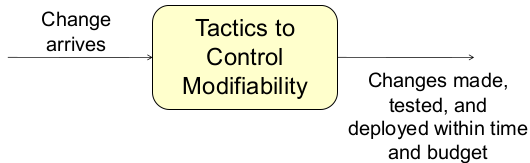
\includegraphics[width=0.5\textwidth]{figures/tacticExample.png}
\caption{Tactic Example Modifiability}
\end{figure}

RECALL: An architectural (style /) pattern expresses a fundamental
structural schema for a software system. It provides a set of predefined
subsystems, specifies their responsibilities, and includes rules and
guidelines for organizing the relationships between them.


\begin{figure}[H]
\centering
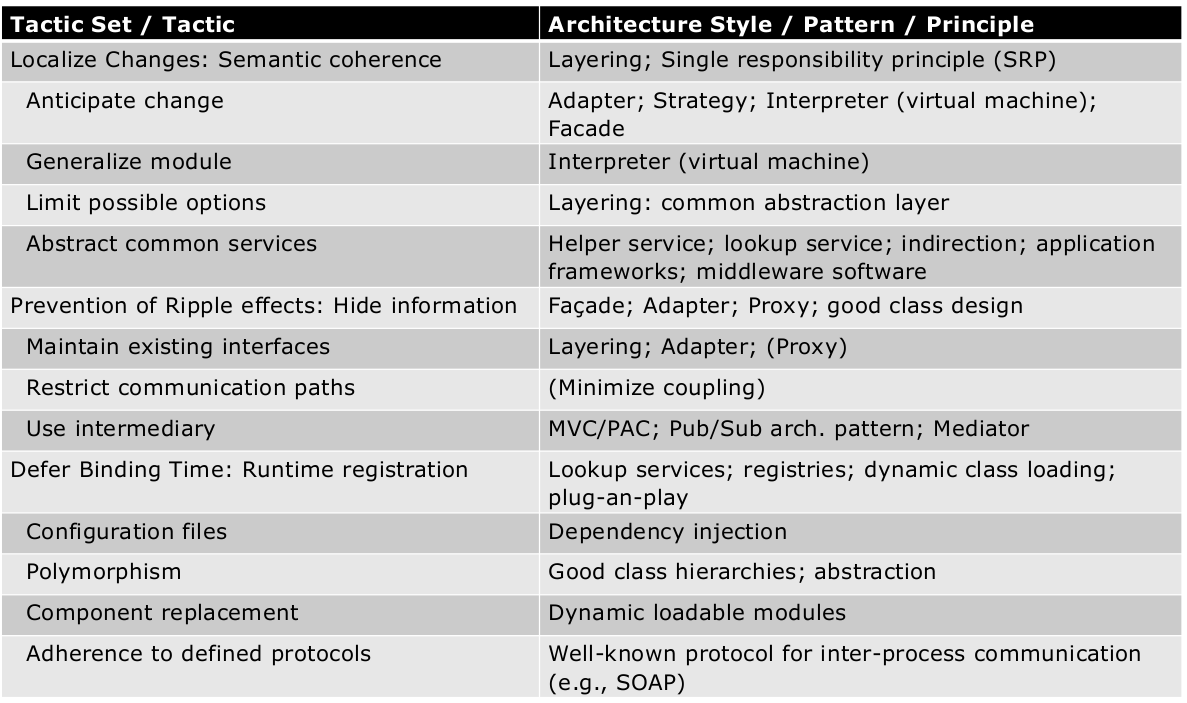
\includegraphics[width=0.5\textwidth]{figures/modifiabilityTactic1.png}
\caption{Modifiability Tactic 1}
\end{figure}

\begin{figure}[H]
\centering
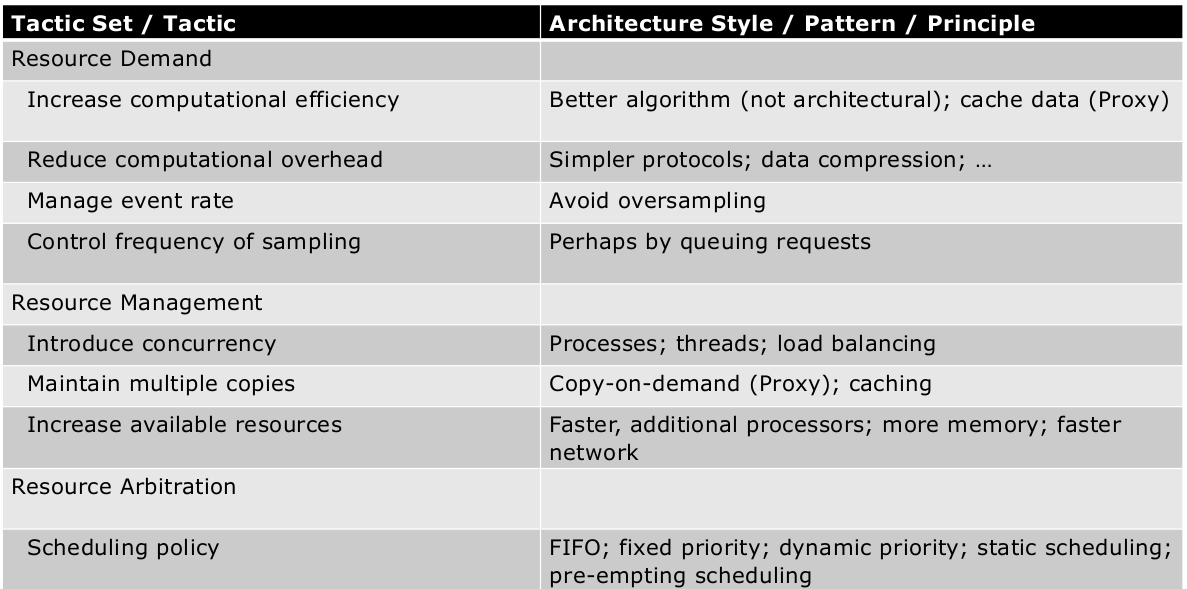
\includegraphics[width=0.5\textwidth]{figures/modifiabilityTactic2.png}
\caption{Modifiability Tactic 2}
\end{figure}

\clearpage